\documentclass[10pt]{article}
\usepackage{icmlko}

\icmlmeta{IP 파운데이션 월드모델}{262}{같은 필드를 한쪽에선 빼고 한쪽에선 쓰고 있었다}{웹툰 ``입장 허들''이 \texttt{daily\_pass} 였다 --- 노트 260이 사후라고 뺀 바로 그 필드}

\begin{document}

\twocolumn[
\icmlheader

\begin{abstract}
노트 261이 남긴 ``성분 대신 토큰'' 갈래를 재다가 딴 것을 봤다. 요일을 일곱
축으로 그냥 주면 판이 0.4943, 성분과 둘 다 주면 0.4971 인데 --- 셋을 짝지어
재니 성분 대 토큰이 $t{=}0.63$ 으로 \textbf{1 SE 안}이라 노트 126의 동점
규칙대로 좁은 쪽(23축)이 남는다. 셋 다 노트 245의 선(0.010) 아래이기도 하다.
그래서 판은 안 바뀌었고, 대신 ``요일이 왜 세나''를 팠다. \textbf{월요일이다}
--- 학습의 21.8\%가 월요일인데 라벨 편차가 $-$0.286 이고 나머지 여섯은
$+$0.045$\sim$$+$0.122 다. 붐비는 슬롯이다. 거기까지 쓰다가
\texttt{webtoon\_axes.py} 를 열었고, 문서 문단에서 이 노트의 진짜 내용을
찾았다. \textbf{웹툰의 ``입장 허들''(\texttt{entry\_friction})이
\texttt{daily\_pass} 다} --- 134행이 \texttt{1.0 if r.get("daily\_pass")
else 0.0} 이다. 노트 260이 메타 축을 만들 때 \emph{바로 그 필드}를
``\texttt{finished} 와 $+$0.841 이라 사후''라고 빼 놓고, 같은 필드가 손 축
다섯 중 하나로 판에 들어와 있었다. 학습의 70.1\%가 \texttt{daily\_pass} 인데
유보는 22.4\% 다 --- \textbf{같은 축이 두 시기에 다른 것을 뜻한다.} 가드 둘이
다 놓쳤다: \textbf{시점}은 축 \emph{이름}에 붙은 뜻(``기획서 태깅'')을 보는데
도메인마다 채우는 원본이 다르고(나머지 여덟은 가격 · 연령이라 사전이다),
\textbf{한철}은 \emph{지표}가 벌어졌는지 보는데 이 축은 덮음이 두 시기 다
100\% 다. 막았다. \textbf{판 0.4916 $\to$ 0.4772}(웹툰 $-$0.0557,
$t{=}-3.09$). 노트 213의 공휴일과 같은 되돌림이다.
\end{abstract}
]

\section{먼저 하던 것: 성분 대신 토큰}

노트 261이 ``요일 일곱을 그냥 일곱 축으로 주면?''을 남겼다. SVD 가 요일의
분산을 여러 성분에 흩는다는 것을 봤으니 자연스러운 물음이다.

\begin{center}\small
\begin{tabular}{lrr}
\hline
 & 축 & 판 \\
\hline
성분 둘(지금) & 23 & 0.4916 \\
토큰 일곱 & 28 & 0.4943 \\
둘 다 & 30 & 0.4971 \\
\hline
\end{tabular}
\quad
\begin{tabular}{lrr}
\hline
짝지어 & 차 & $t$ \\
\hline
성분 $\to$ 토큰 & $+$0.0029 & \textbf{0.63} \\
성분 $\to$ 둘 다 & $+$0.0055 & 1.45 \\
토큰 $\to$ 둘 다 & $+$0.0028 & 1.07 \\
\hline
\end{tabular}
\end{center}

성분 대 토큰이 \textbf{1 SE 안}이다. 노트 126의 동점 규칙 --- 짝지은 1 SE
안이면 좁은 쪽 --- 대로 23축이 남는다. 셋 다 노트 245의 0.010 선 아래이기도
하다. \textbf{안 바꾼다.}

\section{요일이 센 까닭은 월요일이다}

\begin{center}\small
\begin{tabular}{lrrr}
\hline
요일 & 학습 편수 & 몫 & 라벨 편차 \\
\hline
\textbf{월} & 459 & \textbf{21.8\%} & $\mathbf{-0.286}$ \\
화 & 293 & 13.9\% & $+$0.096 \\
수 & 295 & 14.0\% & $+$0.045 \\
목 & 309 & 14.7\% & $+$0.057 \\
금 & 280 & 13.3\% & $+$0.061 \\
토 & 291 & 13.8\% & $+$0.112 \\
일 & 277 & 13.2\% & $+$0.122 \\
\hline
\end{tabular}
\end{center}

월요일만 다르다 --- 편수는 다른 요일의 1.6배인데 라벨이 0.29 낮다. 나머지
여섯은 서로 0.08 안에 모여 있다. \textbf{붐비는 슬롯}이고, 유보에서도
26.4\%로 그대로다.

그리고 연재 \emph{요일 수}는 거의 아무것도 아니다 --- 학습 2,106편 중
2,000편이 주 1회라 편차가 $-$0.001 이다. \textbf{``며칠''에는 분산이 없고
``어느 날''에 있다.} 노트 260이 왜 그렇게 컸는지가 여기서 설명된다.

\section{소스를 열었다가 딴 것을 봤다}

\texttt{venue\_prominence} 가 정말 요일 수인지 확인하려고
\texttt{webtoon\_axes.py} 를 열었다. 문서 문단이 다섯 축을 한 줄씩 적어
놓았는데 두 번째 줄에서 멈췄다.

\begin{quote}\small
\texttt{입장 허들\ \ \ \ 유료 여부(dailyPass).}
\end{quote}

\begin{quote}\small
\texttt{\# 134행} \\
\texttt{a["entry\_friction"] = 1.0 if r.get("daily\_pass") else 0.0}
\end{quote}

\textbf{노트 260이 두 시간 전에 사후라고 뺀 필드다.} 그때 이렇게 적었다 ---
``\texttt{finished} 와 $+$0.841 · 연도와 $-$0.437 이라 완결 표지의 다른
이름이고, \texttt{finished} 는 \texttt{provenance} 에 이미 POST 다.''
메타 축에서는 빼고, 손 축 다섯 중 하나로는 쓰고 있었다.

\begin{figure}[t]
\centering
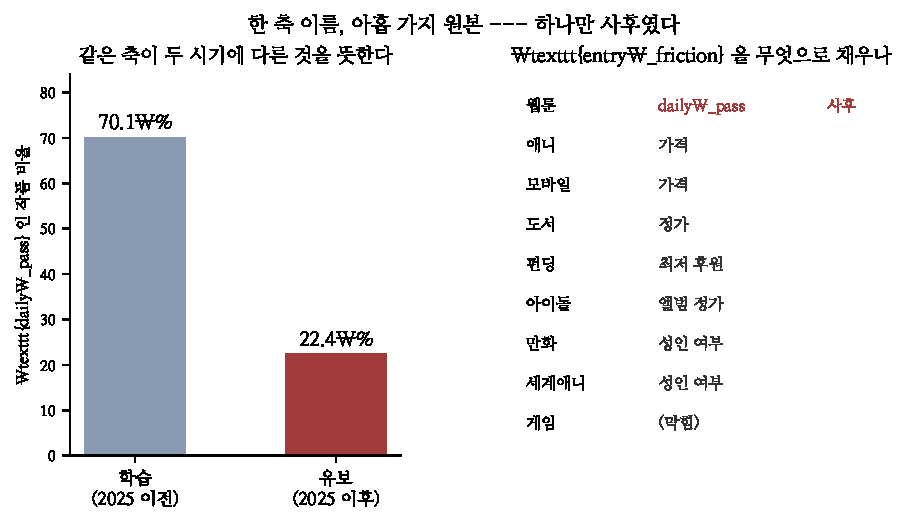
\includegraphics[width=\columnwidth]{figs/fields.pdf}
\caption{왼쪽 --- 시기별 \texttt{daily\_pass} 비율. 오른쪽 --- 도메인마다
같은 축 이름을 무엇으로 채우나.}
\end{figure}

\begin{center}\small
\begin{tabular}{lr}
\hline
웹툰 \texttt{entry\_friction} & \\
\hline
학습(2025 이전) \texttt{daily\_pass} 비율 & \textbf{70.1\%} \\
유보(2025 이후) & \textbf{22.4\%} \\
\hline
\end{tabular}
\end{center}

\textbf{같은 축이 두 시기에 다른 것을 뜻한다.} 학습에서는 ``열에 일곱은
유료''이고 유보에서는 ``열에 둘''이다. 연재가 끝나야 붙는 표지이니 당연하다
--- 유보는 아직 안 끝난 작품들이다.

\section{가드 둘이 왜 놓쳤나}

이 실험실에는 이런 것을 잡으라고 만든 가드가 둘 있는데 다 통과했다.

\paragraph{시점} \texttt{provenance.WHEN} 은 축 \emph{이름}에 뜻을 붙인다
--- \texttt{entry\_friction}: (PRE, ``기획서 태깅''). 그런데 도메인마다
채우는 원본이 다르다.

\begin{center}\small
\begin{tabular}{ll}
\hline
도메인 & \texttt{entry\_friction} 원본 \\
\hline
\textbf{웹툰} & \textbf{\texttt{daily\_pass}} --- 사후 \\
애니 · 모바일 · 도서 & 가격 \\
펀딩 & 최저 후원액 \\
아이돌 & 앨범 정가 \\
만화 · 세계애니 & 성인 여부 \\
게임 & (마스크 0) \\
\hline
\end{tabular}
\end{center}

\textbf{여덟은 사전이고 하나만 사후다.} 이름에 붙인 뜻이 여덟에는 맞고
하나에는 틀렸다. 노트 142가 ``시점은 축의 성질만이 아니다''라며 (축, 도메인)
예외 표를 만들어 뒀는데, 그 표는 \emph{쓰는 쪽}의 예외(모바일 설명문 갱신)만
담고 있었고 \emph{채우는 쪽}의 불일치는 못 담았다.

\paragraph{한철} 노트 214의 한철은 \textbf{지표}가 시기별로 벌어졌는지 본다.
이 축은 덮음이 학습 100\% · 유보 100\% 라 안 걸린다. 한철이 잡는 것은
``유보에서 못 재는 열''이고, 이것은 ``두 시기에 뜻이 다른 열''이다. 다른
병이다.

\section{막았다}

\begin{figure}[t]
\centering

\includegraphics[width=\columnwidth]{figs/board.pdf}
\caption{판의 걸음. 마지막이 이번 되돌림이다.}
\end{figure}

\texttt{lab/fixaxes.py} 에 \texttt{BLOCK} 을 두고 (웹툰,
\texttt{entry\_friction})을 마스크 0 으로 내렸다. 노트 208이 ``확인된 측정
아티팩트를 읽을 때 고친다''고 만들어 둔 자리다.

\begin{center}\small
\begin{tabular}{lrrr}
\hline
 & F21 & F18 & \textbf{F23} \\
\hline
막기 전 & 0.4626 & 0.4875 & \textbf{0.4916} \\
막은 뒤 & 0.4348 & 0.4738 & \textbf{0.4772} \\
\hline
\end{tabular}
\end{center}

웹툰이 0.4768 $\to$ 0.4211($-$0.0557, $t{=}-3.09$)이고 판이 $-$0.0141 이다.
가드 여덟 통과.

\textbf{노트 213과 같은 되돌림이다.} 그때 공휴일 목록을 채우자 0.4603이
0.4396으로 내려앉았고 ``점수가 아니라 자료가 옳아진 것''이라고 적었다.
이번에도 같다. 다만 노트 213은 \emph{빠진 것을 채워서} 내려갔고 이번은
\emph{있던 것을 빼서} 내려갔다.

\paragraph{남은 것}
\begin{center}\small
\begin{tabular}{ll}
\hline
갈래 & 왜 \\
\hline
나머지 축 원본 훑기 & \texttt{entry\_friction} 만 봤다. 넷이 더 있다 \\
채우는 쪽 시점표 & (축, 도메인) $\to$ 원본 필드를 적어 두면 \\
웹툰 대체 축 & 진짜 유료 여부(첫 회 무료 등)가 레코드에 있나 \\
23축 천장 & 막은 뒤로 다시 재야 한다 \\
\hline
\end{tabular}
\end{center}

\paragraph{규약} 축 이름이 아니라 \textbf{채우는 필드}로 시점을 판정한다.
한 이름이 아홉 도메인에서 아홉 가지 필드로 채워지는데, 시점표는 이름 하나에
뜻 하나를 붙이고 있었다. \textbf{내가 한쪽에서 뺀 필드를 다른 쪽에서 쓰고
있지 않은지}가 제일 값싼 확인이다.

\end{document}
